\newpage
\section{Presupuesto del Proyecto}
\label{cap:presupuesto}

Todo proyecto de ingeniería requiere una evaluación de viabilidad económica que cuantifique detalladamente los recursos materiales, lógicos y humanos consumidos durante sus fases de investigación, desarrollo y puesta en marcha. En este capítulo se desglosan los costes asociados al hardware, el licenciamiento de software y la mano de obra, concluyendo con el resumen económico global del proyecto.

\subsection{Costes de hardware y materiales}
\label{sec:costes_hardware}
El coste de adquisición de equipamiento comprende el conjunto de dispositivos físicos, microcontroladores, sensores, actuadores y elementos de conexionado y alimentación necesarios para construir físicamente los tres nodos de instrumentación y el servidor central. En la Tabla~\ref{tbl:presupuesto_hardware} se detalla la lista de materiales (\textit{Bill of Materials}) del prototipo.

\begin{table}[H]
    \centering
    \small
    \renewcommand{\arraystretch}{1.2}
    \setlength{\tabcolsep}{4pt}
    \begin{tabular}{|l|c|c|r|r|}
        \hline
        \textbf{Descripción del componente} & \textbf{Fabricante} & \textbf{Cantidad} & \textbf{Precio Unitario (\euro)} & \textbf{Coste Total (\euro)} \\ \hline
        Raspberry Pi 4 Model B (1\,GB RAM)  & Raspberry Pi  & 1 & 45.00 & 45.00 \\ \hline
        Microcontrolador ESP32 DevKitC v4   & Espressif     & 3 & 6.00  & 18.00 \\ \hline
        Sensor de humedad y temp. DHT11     & Keyes         & 1 & 2.00  & 2.00  \\ \hline
        Fotorresistor LDR (Fotoresistencia)  & Keyes         & 1 & 1.50  & 1.50  \\ \hline
        Relé de estado sólido SSR-25DA 25A  & Fotek         & 1 & 4.00  & 4.00  \\ \hline
        Sensor acústico de alto sonido      & Keyes         & 1 & 3.50  & 3.50  \\ \hline
        Radar FMCW mmWave HLK-LD2410C       & Hi-Link       & 1 & 9.00  & 9.00  \\ \hline
        Diodo emisor láser KY-008           & Keyes         & 1 & 2.00  & 2.00  \\ \hline
        Sensor magnético Reed MC-38         & Keyes         & 1 & 2.00  & 2.00  \\ \hline
        Fuente de alimentación USB-C 5V 3A  & Raspberry Pi  & 1 & 10.00 & 10.00 \\ \hline
        Fuente de alimentación USB 5V 1A    & Genérico      & 3 & 4.00  & 12.00 \\ \hline
        Cajas protectoras y cables Dupont   & Genérico      & 1 & 15.00 & 15.00 \\ \hline
        \textbf{Subtotal Equipamiento}      & --            & -- & --   & \textbf{124.00} \\ \hline
    \end{tabular}
    \caption{Presupuesto desglosado de adquisición de equipos y material de hardware.}
    \label{tbl:presupuesto_hardware}
\end{table}

El coste de adquisición de hardware para la construcción completa del sistema se sitúa en 124.00\,\euro, lo que demuestra la viabilidad económica y el bajo coste del despliegue físico del prototipo de instrumentación.

\subsection{Costes de licencias y software}
\label{sec:costes_software}
Para garantizar la sostenibilidad, la privacidad y evitar la dependencia de licencias comerciales recurrentes de pago (modelo *Software as a Service*), se ha diseñado la arquitectura lógica basándose en su totalidad en software libre, de código abierto o licencias de uso no comercial de carácter gratuito. El coste desglosado de licenciamiento de software se expone en la Tabla~\ref{tbl:presupuesto_software}.

\begin{table}[H]
    \centering
    \small
    \renewcommand{\arraystretch}{1.2}
    \setlength{\tabcolsep}{6pt}
    \begin{tabular}{|l|c|c|c|}
        \hline
        \textbf{Software / Plataforma} & \textbf{Tipo de Licencia} & \textbf{Uso en el Proyecto} & \textbf{Coste (\euro)} \\ \hline
        Raspberry Pi OS (Debian)       & Código Abierto (GPL)      & Sistema operativo host      & 0.00 \\ \hline
        Docker Community Edition       & Código Abierto (Apache)   & Orquestación de contenedores& 0.00 \\ \hline
        Portainer Community Edition    & Libre con restricciones   & Panel de control Docker     & 0.00 \\ \hline
        Home Assistant Container       & Código Abierto (Apache)   & Orquestador domótico central& 0.00 \\ \hline
        ESPHome suite                  & Código Abierto (MIT/GPL)  & Compilador cruzado firmware  & 0.00 \\ \hline
        Base de datos SQLite           & Dominio Público           & Motor de almacenamiento HA  & 0.00 \\ \hline
        VPN Tailscale (Free tier)      & Comercial Gratuita        & Acceso remoto cifrado       & 0.00 \\ \hline
        \textbf{Subtotal Licencias}    & --                        & --                          & \textbf{0.00} \\ \hline
    \end{tabular}
    \caption{Presupuesto de licencias de software y plataformas lógicas.}
    \label{tbl:presupuesto_software}
\end{table}

El uso del ecosistema de software libre y de código abierto permite mitigar a cero los costes lógicos del sistema, garantizando la total autonomía tecnológica y eliminando las cuotas mensuales de persistencia en la nube presentes en entornos domóticos propietarios.

\subsection{Costes de operación y mantenimiento}
\label{sec:costes_operacion}
Los costes recurrentes de operación y mantenimiento comprenden el coste eléctrico derivado del funcionamiento continuo del prototipo (Raspberry Pi activa 24/7 y microcontroladores ESP32 alimentados permanentemente) y la amortización del equipamiento hardware:
\begin{itemize}
    \item \textbf{Consumo eléctrico anual:} calculado en el Capítulo~\ref{cap:evaluacion_sistema} en base al perfil de potencia medio de $5.15$\,W de la instalación y un precio medio de electricidad de $0.20$\,\euro/kWh, lo que arroja un coste operativo de **$9.02$\,\euro/año**.
    \item \textbf{Amortización del equipamiento:} estimando una vida útil del prototipo físico de 5 años con depreciación lineal, el coste anual de amortización se modela como:
    \begin{equation}
        \text{Amortización} = \frac{\text{Coste de Equipamiento}}{\text{Vida Útil}} = \frac{124.00\,\text{\euro}}{5\,\text{años}} = 24.80\,\text{\euro/año}
    \end{equation}
\end{itemize}
El coste operativo y de mantenimiento estimado para el primer año se sitúa en un total de **$33.82$\,\euro/año** (suma del consumo eléctrico y la amortización).

\subsection{Mano de obra y resumen económico}
\label{sec:mano_obra_resumen}
El principal factor económico en el desarrollo del Trabajo Fin de Grado corresponde a las horas de diseño, programación, soldadura física, calibración y pruebas invertidas por el desarrollador. Se estiman un total de 300 horas dedicadas a la materialización del proyecto. Valorando el coste por hora de un ingeniero técnico de software junior en $25.00$\,\euro/hora, el coste de la mano de obra se desglosa en la Tabla~\ref{tbl:mano_obra}.

\begin{table}[H]
    \centering
    \small
    \renewcommand{\arraystretch}{1.2}
    \setlength{\tabcolsep}{8pt}
    \begin{tabular}{|l|c|c|r|}
        \hline
        \textbf{Fase de ingeniería} & \textbf{Horas dedicadas} & \textbf{Precio/Hora (\euro)} & \textbf{Coste total (\euro)} \\ \hline
        Investigación y análisis    & 60  & 25.00 & 1\,500.00 \\ \hline
        Diseño y arquitectura       & 50  & 25.00 & 1\,250.00 \\ \hline
        Montaje y conexionado físico& 40  & 25.00 & 1\,000.00 \\ \hline
        Desarrollo e integración    & 100 & 25.00 & 2\,500.00 \\ \hline
        Validación y plan de pruebas& 50  & 25.00 & 1\,250.00 \\ \hline
        \textbf{Total Mano de Obra} & \textbf{300} & --    & \textbf{7\,500.00} \\ \hline
    \end{tabular}
    \caption{Presupuesto estimado de mano de obra en ingeniería y desarrollo.}
    \label{tbl:mano_obra}
\end{table}

A partir de los tres subgrupos anteriores (hardware, software y mano de obra), se realiza la consolidación del presupuesto total del proyecto domótico, presentándose el balance general en la Tabla~\ref{tbl:resumen_presupuesto}.

\begin{table}[H]
    \centering
    \small
    \renewcommand{\arraystretch}{1.2}
    \setlength{\tabcolsep}{10pt}
    \begin{tabular}{|l|r|}
        \hline
        \textbf{Concepto Presupuestario} & \textbf{Coste Parcial (\euro)} \\ \hline
        Equipos y material de hardware    & 124.00 \\ \hline
        Licencias y plataformas de software & 0.00 \\ \hline
        Mano de obra (ingeniería de desarrollo) & 7\,500.00 \\ \hline
        \textbf{Presupuesto de Ejecución Material (PEM)} & \textbf{7\,624.00} \\ \hline
        Impuesto sobre el Valor Añadido (IVA, 21\,\%) & 1\,601.04 \\ \hline
        \textbf{PRESUPUESTO TOTAL (IVA INCLUIDO)} & \textbf{9\,225.04} \\ \hline
    \end{tabular}
    \caption{Resumen económico consolidado del proyecto domótico.}
    \label{tbl:resumen_presupuesto}
\end{table}

La distribución porcentual de los costes de ejecución del proyecto se representa gráficamente en la Figura~\ref{fig:distribucion_costes}.

\begin{figure}[H]
    \centering
    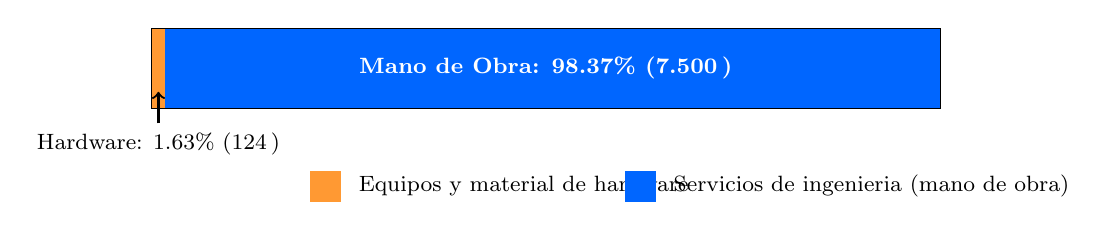
\begin{tikzpicture}
        % Barra exterior (contenedor)
        \draw[thick, fill=gray!10] (0,0) rectangle (10,1);
        
        % Segmento Hardware (1.63% de 10cm es 0.16cm)
        \fill[orange!80!white] (0,0) rectangle (0.16,1);
        
        % Segmento Mano de Obra (98.37% de 10cm es 9.84cm)
        \fill[blue!60!cyan] (0.16,0) rectangle (10,1);
        
        % Etiquetas y lineas indicadoras
        % Hardware
        \draw[thick, ->] (0.08, -0.2) -- (0.08, 0.2);
        \node[anchor=north, font=\footnotesize] at (0.08, -0.2) {Hardware: 1.63\% (124\,\euro)};
        
        % Mano de obra
        \node[font=\footnotesize\bfseries, color=white] at (5, 0.5) {Mano de Obra: 98.37\% (7.500\,\euro)};
        
        % Leyenda
        \fill[orange!80!white] (2, -1.2) rectangle (2.4, -0.8);
        \node[anchor=west, font=\footnotesize] at (2.5, -1) {Equipos y material de hardware};
        
        \fill[blue!60!cyan] (6, -1.2) rectangle (6.4, -0.8);
        \node[anchor=west, font=\footnotesize] at (6.5, -1) {Servicios de ingenieria (mano de obra)};
    \end{tikzpicture}
    \caption{Distribución porcentual de los costes del proyecto entre equipamiento y mano de obra.}
    \label{fig:distribucion_costes}
\end{figure}